% =====================================================================================
% EXPERIMENTAL VALIDATION -- results section (IEEEtran, two-column)
% Data   : results/scenario_P01_adaptive_{collaborative_20261009_035710, assistive_20261009_040743,
%          solo_20261009_040950, collaborative_20261009_041509}  (*_data.csv, *_events.csv, *_metrics.csv)
% Figure : results/figures_20261009_045346/fig_combined.pdf  (plotScenariosHRC)
% Every number below was computed from these logs (time-weighted by the real epoch durations).
% Packages: graphicx, booktabs, multirow, amsmath.  Replace the \ref / \cite keys with your own labels.
% =====================================================================================

\section{Experimental Validation}
\label{sec:results}

The proposed framework was validated on a physical human--robot workcell in which a worker performs an
assembly task while a collaborative manipulator operates in the three interaction modes encoded in the
POMDP: solo, assistive, and collaborative. The experiments were designed to verify that the decision-making
framework 1) adapts the robot behavior to the estimated mental fatigue, physical fatigue, and attention of
the worker; 2) does so in a context-dependent manner, i.e., according to the interaction mode and the
human--robot separation; and 3) preserves human safety at all times, while every speed reduction remains
traceable to the human or environmental factor that caused it.

\subsection{Experimental Setup}
\label{sec:setup}

\begin{figure}[!t]
\centering
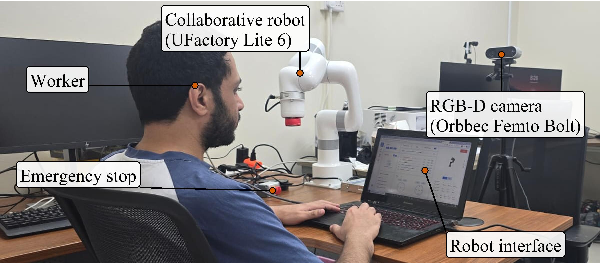
\includegraphics[width=\columnwidth]{setup_figure/fig_setup_wide.pdf}
\caption{Experimental workcell. The RGB-D camera observes the worker and the collaborative robot; the
human-state estimates and the safety geometry computed from its stream are used by the POMDP decision layer,
which commands the robot. An emergency stop remains within the worker's reach.}
\label{fig:setup}
\end{figure}

The workcell comprises a six-degree-of-freedom UFactory Lite~6 collaborative arm and a single Orbbec Femto
Bolt RGB-D camera that observes the whole workstation (Fig.~\ref{fig:setup}). The camera frame was registered
to the robot base by hand--eye calibration with a root-mean-square residual of 3.8~mm (maximum 5.8~mm).
The workspace is partitioned into a storage area (two storage boxes localized by color segmentation),
a handover point, and a shared assembly area. From the RGB-D stream, the human-state estimation module
(Section~\ref{sec:estimation}) provides, at 6.8--9.1~Hz, the mental-fatigue observation $F_m$, the
physical-fatigue observation $F_p$, the attention observation $A$ together with the continuous look-away
time, an estimate confidence, and the three-dimensional positions of the hand and upper limb. These
quantities are fused with the measured robot configuration to compute the hand--tool distance $d_h$ and
the minimum clearance $c$ between the tracked palm and the robot links.

The decision layer executes the QMDP policy of Section~\ref{sec:pomdp} over $34\,992$ states and ten
actions, obtained offline by value iteration ($\gamma = 0.95$), and maintains online the belief over
$(F_p, F_m, A)$. The planner action is processed by the fatigue-adaptation and worker-dialogue layer, the
safety supervisor, and the solo fatigue--distance speed law (Section~\ref{sec:architecture}). Robot motions
are executed as joint-space waypoint sequences with blended segments, so that the commanded joint speed is
constant between waypoints and any change of speed is attributable to a decision. Three speed levels are
used: slow ($5^\circ$/s), normal ($23^\circ$/s), and fast ($30^\circ$/s); the fast level is reserved for
retreat motions directed away from the worker. The safety parameters are: collaborative envelope
$d_h \le 0.35$~m; active-risk clearance $c < 0.05$~m; solo separation clearance $c \ge 0.30$~m; and release
of a protective stop only after $c \ge 0.06$~m and $d_h \ge 0.15$~m hold for two consecutive epochs. At every
decision epoch, the observation, the sustained fatigue level, the planner (nominal) action, the executed
action, the commanded and measured joint speeds, the safety geometry, and the cause of any speed reduction
were logged.

\subsection{Protocol}
\label{sec:protocol}

Because fatigue manifests differently across individuals, all fatigue observations are referred to
participant-specific baselines recorded before the experiment: a 60-s facial baseline (eye-aspect and
mouth-aspect ratio statistics) for the mental-fatigue estimator, a postural baseline for the
physical-fatigue index, and a 20-s calibration of the assembly area.

The objective of the experiment is to evaluate the decision-making framework over the full range of human
states, i.e., low, medium, and high fatigue and focused, uncertain, and distracted attention, including the
transitions between them. Reaching high fatigue naturally would require hours of sustained work and would
not produce repeatable transitions. The participant therefore deliberately enacted, at chosen moments, the
behavioral indicators that the estimation module associates with mental fatigue and reduced attention:
yawning, prolonged eye closures, intentional task errors, reduced focus on the task, and gaze departures
from the shared workspace. Because the decision layer acts on the estimated human state, these cues
exercise the policy through the same sensing and estimation pathway that natural fatigue follows, while
the timing and intensity of each condition remain under experimental control. The participant then
performed four consecutive sessions covering all interaction modes:
\begin{itemize}
\item \textit{Session I -- Collaborative} (547.6~s): the robot works with the participant in the shared
assembly area.
\item \textit{Session II -- Assistive} (93.5~s): the participant requests a tool; the robot fetches it from
the storage area, delivers it at the handover point, and returns to its safe position.
\item \textit{Session III -- Solo} (212.4~s): the robot performs pick-and-place transfers between the two
storage boxes while the participant assembles at the adjacent workstation.
\item \textit{Session IV -- Collaborative with attention lapses} (117.3~s): the participant enacted
pronounced fatigue cues and repeated gaze departures from the shared workspace to drive the estimated state
to high fatigue and distraction and, when prompted by the rest warning, chose to rest.
\end{itemize}
In total, 970.8~s of physical interaction and 804 decision epochs were recorded with the proposed adaptive
framework in the loop.

\subsection{Evaluation Metrics}
\label{sec:metrics}

Five groups of metrics were computed from the logs, time-weighted by the actual epoch durations:
\begin{enumerate}
\item \textit{Speed-mode occupancy}: share of time at nominal speed (commanded speed $\ge 23^\circ$/s),
reduced speed ($0 < \dot q_{\mathrm{cmd}} < 23^\circ$/s), stationary hold or wait, and protective stop; and
the mean commanded joint speed $\bar v$ while moving.
\item \textit{Safety margins}: the minimum hand--tool distance $d_h^{\min}$ and the minimum palm--robot
clearance $c^{\min}$ over all epochs with commanded motion, and the number of epochs in which the robot
was commanded to move with $c < 0.05$~m or with an unverified safety geometry.
\item \textit{Responsiveness}: the delay between a change of the observed human state and the corresponding
change of the executed action.
\item \textit{State-conditioned decision consistency}: the distribution of the planner actions conditioned
on the observed human state.
\item \textit{Decision attribution}: each epoch with a reduced speed is assigned to a single cause, following
the order of authority of the decision layers: fatigue level, fatigue $+$ distance, distance, attention,
low estimate confidence, sensing, and planner belief.
\end{enumerate}

% -------------------------------------------------------------------------------------
\begin{figure*}[!t]
\centering
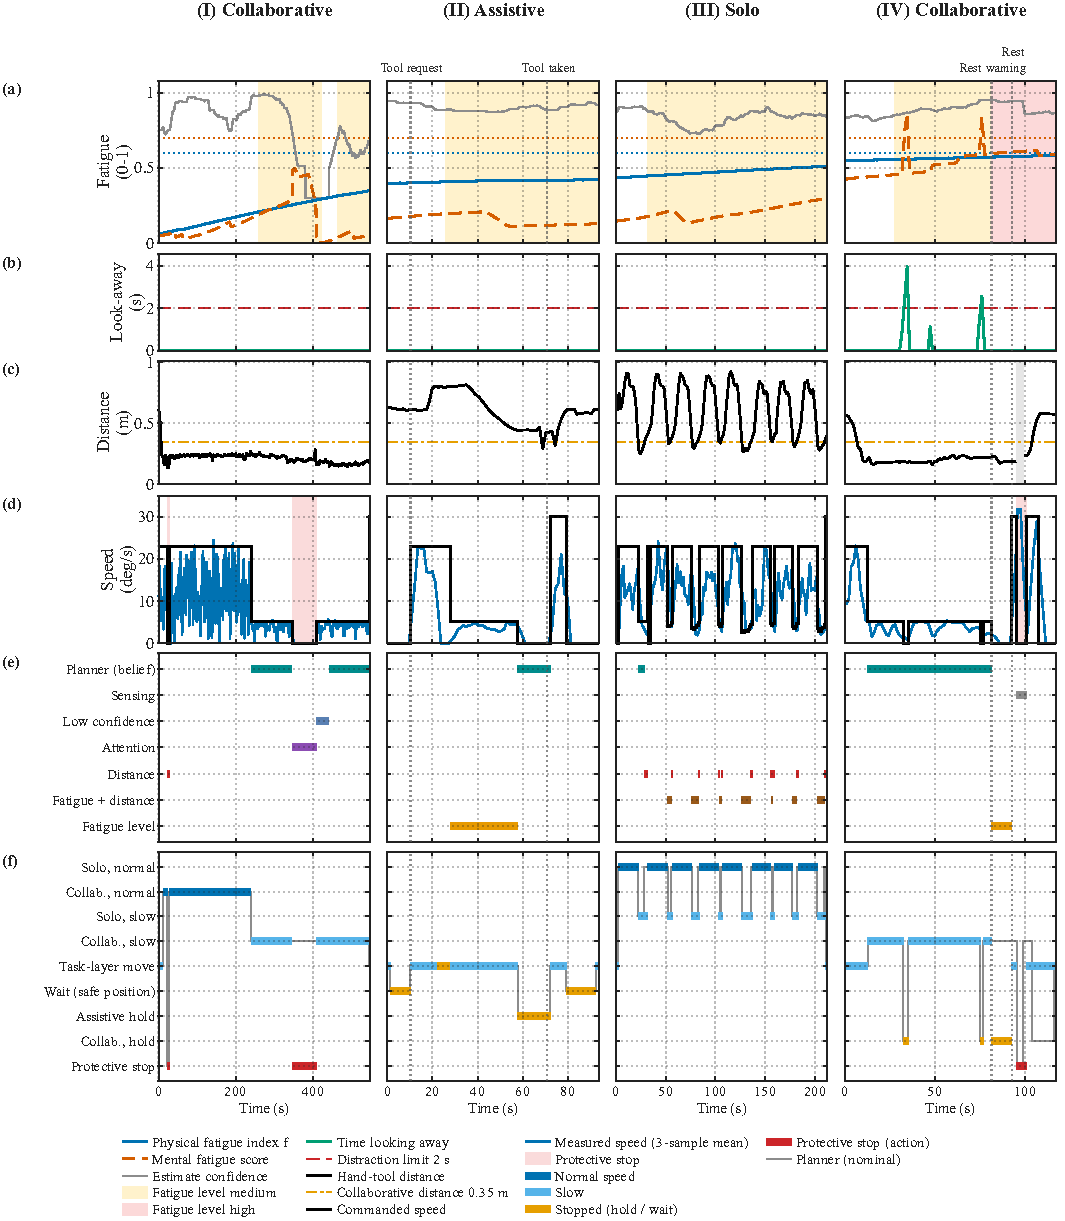
\includegraphics[width=\textwidth]{figures_20261009_045346/fig_combined.pdf}
\caption{Human state, safety geometry, and robot decisions in the four experimental sessions: (I)
collaborative, (II) assistive, (III) solo, and (IV) collaborative with attention lapses and a rest. (a)
Physical-fatigue index, mental-fatigue score, and confidence of the human-state estimate; the background
shading marks the sustained fatigue level (medium/high) computed from the belief. (b) Continuous look-away
time and the 2-s distraction limit. (c) Hand--tool distance and the 0.35-m collaborative envelope. (d)
Commanded joint speed (black) and measured joint speed (blue); red shading marks protective stops. (e) Cause
of every speed reduction, as attributed by the decision layers. (f) Executed action, colored by speed level
(normal, slow, stationary, protective stop), with the planner (nominal) action in gray. Event markers at the
top indicate the worker requests and the dialogue events.}
\label{fig:sessions}
\end{figure*}
% -------------------------------------------------------------------------------------

\subsection{Session-Level Results}
\label{sec:session_results}

Fig.~\ref{fig:sessions} reports the complete time evolution of the human state, the safety geometry, and the
robot decisions for the four sessions, and Table~\ref{tab:sessions} summarizes the corresponding metrics.

\begin{table}[!t]
\centering
\caption{Summary of the Four Experimental Sessions}
\label{tab:sessions}
\setlength{\tabcolsep}{4pt}
\renewcommand{\arraystretch}{1.08}
\begin{tabular}{@{}lcccc@{}}
\toprule
 & \textbf{I} & \textbf{II} & \textbf{III} & \textbf{IV} \\
Interaction mode & Collab. & Assist. & Solo & Collab. \\
\midrule
Duration (s) & 547.6 & 93.5 & 212.4 & 117.3 \\
Decision epochs & 505 & 71 & 145 & 83 \\
\midrule
\multicolumn{5}{@{}l}{\textit{Human state}} \\
Mental-fatigue score (range) & 0.00--0.50 & 0.11--0.21 & 0.13--0.30 & 0.42--0.86 \\
Physical-fatigue index (start$\to$end) & 0.06$\to$0.35 & 0.40$\to$0.42 & 0.43$\to$0.51 & 0.55$\to$0.58 \\
Maximum sustained fatigue level & Medium & Medium & Medium & High \\
Look-aways $>2$~s & 0 & 0 & 0 & 2 \\
\midrule
\multicolumn{5}{@{}l}{\textit{Robot behavior (\% of session time)}} \\
Nominal/fast speed & 43.0 & 26.4 & 71.6 & 18.8 \\
Reduced speed & 44.4 & 31.9 & 26.5 & 54.9 \\
Stationary (hold/wait) & 0.0 & 41.6 & 1.9 & 21.8 \\
Protective stop & 12.6 & 0.0 & 0.0 & 4.6 \\
Mean commanded speed $\bar v$ ($^\circ$/s) & 13.9 & 14.1 & 17.9 & 10.3 \\
\midrule
\multicolumn{5}{@{}l}{\textit{Safety (epochs with commanded motion)}} \\
Protective stops & 2 & 0 & 0 & 1 \\
$d_h^{\min}$ (m) & 0.143 & 0.317 & 0.249 & 0.161 \\
$c^{\min}$ (m) & 0.053 & 0.227 & 0.159 & 0.071 \\
Motion with $c < 0.05$~m & 0 & 0 & 0 & 0 \\
Motion with unverified geometry & 0 & 0 & 0 & 0 \\
\bottomrule
\end{tabular}
\end{table}

\subsubsection{Collaborative Operation Across Mental-Fatigue Levels (Session I)}
After the transfer to the assembly area, the planner selected collaborative work at normal speed while the
mental-fatigue observation remained low [Fig.~\ref{fig:sessions}(I)]. At $t = 22.9$~s, the participant's
hand approached the tool and the palm--robot clearance dropped to 0.047~m, below the active-risk threshold.
The protective stop was issued in the same epoch in which the violation was detected, and the measured
joint speed remained zero throughout the stop. The closest approach of the whole session ($d_h = 0.132$~m, $c = 0.042$~m, $t = 25.8$~s) therefore
occurred while the robot was already stationary. The stop was released at $t = 28.9$~s, only after the
release clearances had been verified for two consecutive epochs, and normal-speed collaboration resumed.

At $t = 237.1$~s, the mental-fatigue observation changed from low to medium with respect to the
participant's baseline. The belief-based policy switched from collaborative-normal to collaborative-slow
at $t = 240.2$~s, i.e., within three decision epochs (3.1~s), reducing the commanded speed from $23$ to
$5^\circ$/s ($-78\%$). Notably, the persistence-filtered sustained fatigue level, which drives the
rule-based fatigue adaptation, reached medium only at $t = 258.7$~s: the POMDP policy responded
18.5~s earlier than the deterministic adaptation layer. This result shows that the belief update, rather than
a fixed threshold, is the primary adaptation mechanism, and that the downstream rules act as a consistent
backstop. Because the speed levels scale the same joint-space path uniformly in time, the Cartesian
velocity of every robot point scales by the same factor; the slow collaborative action therefore reduces the
kinetic energy of the robot along its path by $1 - (5/23)^2 \approx 95\%$ relative to the nominal motion.

Later in the session, the participant's face became unobservable while the hand remained within the
collaborative envelope ($d_h \approx 0.20$~m). Since attention could not be confirmed at close range, the
safety supervisor commanded a protective stop at $t = 346.5$~s (cause: attention) and maintained it until
attention was observed again and the release conditions were satisfied ($t = 409.9$~s). During the
subsequent interval in which the mental-fatigue estimate was not yet available (confidence $\le 0.5$), the
framework retained the conservative slow action instead of reverting to normal speed (cause: low
confidence, 32~s). From $t = 441.8$~s onward, the estimate again reported medium mental fatigue, and the
planner kept the slow collaborative action until the end of the session.

\subsubsection{Fatigue-Aware Assistance (Session II)}
Upon the tool request ($t = 10.3$~s), the robot fetched and grasped the tool at normal speed
(10.3--26.8~s), since these motions take place in the storage area, far from the participant
($d_h \ge 0.60$~m). The sustained fatigue level reached medium at $t = 25.6$~s; consequently, the approach
toward the handover point, the only phase that brings the robot toward the worker, was executed at
$5.06^\circ$/s, i.e., the nominal speed scaled by the fatigue-dependent approach factor $5/23$ (cause:
fatigue level, 30~s). The robot then remained stationary at the handover point while the participant took
the tool ($t = 70.8$~s) and retreated to its safe position at the fast level ($30^\circ$/s), a motion that
increases the separation and minimizes the exposure time. The assistive cycle was completed without any
protective stop, with $d_h^{\min} = 0.317$~m and $c^{\min} = 0.227$~m during motion.

\subsubsection{Context-Dependent Adaptation in Solo Operation (Session III)}
In solo mode, the participant's hand periodically approached the robot path during the assembly
[Fig.~\ref{fig:sessions}(III)(c)], while the sustained fatigue level was medium from $t = 31.4$~s and the
physical-fatigue index increased from 0.43 to 0.51. Despite this fatigue level, the planner selected the
solo-normal action in 117 of 143 decisions (81.8\%), whereas, in collaborative mode, a medium fatigue
observation led to the slow action in 98.7\% of the decisions (Table~\ref{tab:policy}). This contrast is the
intended context dependence of the reward: the fatigue cost is weighted by the interaction level of the mode
($\lambda_s = 0$, $\lambda_a = 0.6$, $\lambda_c = 1.0$), and in solo mode fatigue penalizes only motion close
to the worker. Accordingly, whenever the palm--robot clearance fell below the 0.30-m separation clearance
with medium fatigue, the fatigue--distance law reduced the commanded speed in proportion to the clearance,
from $4.2^\circ$/s at $c = 0.259$~m to $2.6^\circ$/s at $c = 0.178$~m (cause: fatigue $+$ distance, 33~s),
and restored the nominal speed as soon as the separation was verified again. As a result, the robot
operated at nominal speed during 71.6\% of the session and maintained a mean commanded speed of
$17.9^\circ$/s (78\% of nominal), with no protective stop and $c^{\min} = 0.159$~m.

\subsubsection{Attention Lapses, High Fatigue, and Rest (Session IV)}
Session IV started with an elevated mental-fatigue estimate (score 0.42, rising to 0.86) and the highest
physical-fatigue index of the experiment (0.55--0.58). On arrival in the assembly area ($t = 12.7$~s), the
planner selected collaborative-slow and never selected normal-speed collaboration in this session
[Fig.~\ref{fig:sessions}(IV)]. Brief glances away from the workspace (0.9, 1.1, and 1.3~s) were classified as
uncertain attention and did not interrupt the task, which avoids nuisance stops. When the look-away time
exceeded the 2-s limit ($t = 32.5$~s, peak 3.9~s; $t = 75.3$~s, peak 2.6~s), the planner selected the
collaborative hold in the same epoch, and the robot resumed slow collaboration as soon as the gaze returned
to the workspace ($t = 35.3$ and $77.0$~s). These holds were selected by the POMDP policy itself from the
attention component of the belief (Table~\ref{tab:policy}), while the safety supervisor remained available as
an independent backstop.

At $t = 81.5$~s, the sustained fatigue level became high. The rest warning was displayed in the same
epoch, and the robot was held stationary until the worker answered. The participant chose to rest
($t = 92.7$~s), and the robot immediately retreated to its safe position at the fast level. During the
retreat, the tracked geometry exceeded its validity age ($t = 95.4$~s); the supervisor then commanded a
protective stop (cause: sensing) and released it only after the geometry had been verified again
($t = 100.8$~s), after which the retreat was completed and the robot waited at its safe position until the
end of the rest.

\subsection{State-Conditioned Decision Consistency}
\label{sec:policy_consistency}

Table~\ref{tab:policy} reports the distribution of the planner actions during collaborative work (Sessions I
and IV, 566 decisions) conditioned on the observed human state. The policy exhibits a clear, graded mapping
from human state to robot behavior: normal speed was selected in 98.6\% of the decisions under low mental
fatigue, slow collaboration in 98.7\% under medium fatigue, and, under high fatigue, the policy never
selected normal speed and complemented slow collaboration with holds and stops. The only normal-speed
decisions under medium fatigue (1.3\%) are the three epochs immediately following the low-to-medium
transition at $t = 237.1$~s, which reflects the Bayesian filtering of the belief: a single observation does
not switch the policy, whereas consistent evidence does within seconds. The stops selected under low and
high fatigue coincide exactly with the epochs of observed active-interaction risk and of unverified
geometry, respectively. When mental fatigue was unobservable, the policy selected the slow action in all
cases, and every look-away longer than 2~s produced a hold, whereas shorter glances never did.

\begin{table}[!t]
\centering
\caption{Planner Actions in Collaborative Work Conditioned on the Observed Human State (Sessions I and IV)}
\label{tab:policy}
\setlength{\tabcolsep}{4.5pt}
\renewcommand{\arraystretch}{1.08}
\begin{tabular}{@{}lccccc@{}}
\toprule
 & & \multicolumn{4}{c}{\textbf{Planner action (\% of decisions)}} \\
\cmidrule(l){3-6}
\textbf{Observed state} & $n$ & Normal & Slow & Hold & Stop \\
\midrule
$F_m$ low & 211 & \textbf{98.6} & 0.0 & 0.0 & 1.4$^{a}$ \\
$F_m$ medium & 228 & 1.3$^{b}$ & \textbf{98.7} & 0.0 & 0.0 \\
$F_m$ high & 73 & 0.0 & \textbf{80.8} & 13.7 & 5.5$^{c}$ \\
$F_m$ unobservable & 54 & 0.0 & \textbf{100} & 0.0 & 0.0 \\
\midrule
Look-away $<2$~s & 5 & 0.0 & \textbf{100} & 0.0 & 0.0 \\
Look-away $\ge 2$~s & 3 & 0.0 & 0.0 & \textbf{100} & 0.0 \\
\bottomrule
\multicolumn{6}{@{}p{0.95\columnwidth}@{}}{\footnotesize $^{a}$Epochs with observed active-interaction risk
($c < 0.05$~m). $^{b}$The three epochs following the low-to-medium transition. $^{c}$Epochs with unverified
safety geometry. The attention rows are a subset of the $F_m$ rows.}
\end{tabular}
\end{table}

\subsection{Safety Outcomes}
\label{sec:safety}

Across the 970.8~s of interaction, the robot was never commanded to move while the palm--robot clearance was
below the 0.05-m active-risk threshold or while the safety geometry was unverified (Table~\ref{tab:sessions}).
The smallest clearance during motion (0.053~m) occurred in collaborative work at the slow level, and the
smallest separation of the entire experiment ($c = 0.042$~m) was reached while the robot was already in a
protective stop. The three protective stops covered the three distinct hazard classes handled by the
supervisor, namely proximity (Session I), unconfirmed attention at close range (Session I), and degraded
sensing (Session IV), and each of them was released only after the release conditions had been verified.
In the assistive and solo modes, the fatigue-dependent speed laws kept the separation large enough that no
protective stop was required.

These outcomes result from the layered structure of the framework. The POMDP policy anticipates risk by
lowering the speed as soon as the belief indicates fatigue or inattention, so that, when a hazard does
materialize, the robot is already moving slowly: the robot was moving at $2$--$4^\circ$/s when the attention
stop of Session I and the attention holds of Session IV were issued. The safety supervisor then provides a
deterministic guarantee that is independent of the estimate of the human state.

\subsection{Transparency of Speed Adaptation}
\label{sec:transparency}

Every reduced-speed epoch of the experiment (416 of 416) was attributed to an identified cause.
Table~\ref{tab:causes} summarizes the attributed time per session. The distribution of causes reflects the
operating context. In collaborative work, the reductions were driven by the planner belief on fatigue and
attention (Sessions I and IV), complemented by attention, low-confidence, and sensing safeguards. In
assistive mode, the speed was reduced only during the approach toward the worker (fatigue level) and the
stationary handover (planner). In solo mode, it was confined to
the intervals in which a fatigued worker came close to the robot (fatigue $+$ distance and distance). This
attribution, displayed online and recorded at every epoch [Fig.~\ref{fig:sessions}(e)], makes each adaptation
of the robot explainable to the worker and auditable after the task.

\begin{table}[!t]
\centering
\caption{Attribution of the Robot Speed Reductions (Cumulative Time, s)}
\label{tab:causes}
\setlength{\tabcolsep}{5pt}
\renewcommand{\arraystretch}{1.08}
\begin{tabular}{@{}lcccc@{}}
\toprule
\textbf{Cause} & \textbf{I} & \textbf{II} & \textbf{III} & \textbf{IV} \\
\midrule
Planner belief & 211 & 14 & 6 & 69 \\
Fatigue level & -- & 30 & -- & 11 \\
Fatigue $+$ distance (solo) & -- & -- & 33 & -- \\
Distance & 6 & -- & 17 & -- \\
Attention & 63 & -- & -- & -- \\
Low estimate confidence & 32 & -- & -- & -- \\
Sensing & -- & -- & -- & 5 \\
\midrule
Attributed reduced-speed epochs & 284/284 & 33/33 & 37/37 & 62/62 \\
\bottomrule
\end{tabular}
\end{table}

\subsection{Discussion}
\label{sec:discussion}

The experimental results support the three claims of this work. First, the proposed POMDP translates the
estimated mental fatigue, physical fatigue, and attention into graded robot behaviors (normal, slow, hold,
stop, and rest-oriented retreat), and it responds to changes of the human state within seconds and ahead of
threshold-based rules, as shown by the anticipated slowdown of Session I and the attention holds of Session
IV. Second, the adaptation is context-dependent: the same medium fatigue level slowed the robot in 98.7\% of
the collaborative decisions but in solo mode only when the worker came close, which preserved 71.6\% of
nominal-speed operation and avoided unnecessary productivity losses. Third, safety was preserved in all
modes: no motion was commanded below the active-risk clearance or without verified geometry, the closest
human--robot approach occurred with the robot stationary, and every protective stop and speed reduction was
attributed to an explicit cause. Because the human-state conditions were elicited in a controlled manner, these
behaviors were observed across every fatigue and attention level and every interaction mode within a single
experimental campaign. Together with the participant-specific baselines, these properties make the
framework suitable for industrial workcells in which the human state varies over time and across workers.
